\documentclass[11pt, norsk]{article}
%\usepackage[latin1]{inputenc}
\usepackage[T1]{fontenc}
\usepackage[utf8]{inputenc}
\usepackage[norsk]{babel}   % S P R A A K


% \usepackage{graphicx}    % postscript graphics
\usepackage{amssymb, amsmath, amsthm, amssymb} % symboler, osv
\usepackage{mathrsfs}
\usepackage{url}
\usepackage{thmtools}
\usepackage{enumerate}  % lister $  
\usepackage{float}
\usepackage{tikz}
\usetikzlibrary{calc}
\usepackage{tikz-3dplot}
\usepackage{subcaption}
\usepackage[all]{xy}   % for comm.diagram
\usepackage{wrapfig} % for float right
\usepackage{hyperref}
\usepackage{mystyle} % stilfilen      


\begin{document}
\title{Oppgaver MAT2500}
\author{Fredrik Meyer}
\maketitle 

\begin{oppg}
La $K$ være et tredimensjonalt konvekst polyeder. La $V_K$ være mengden av hjørner, $E_K$ mengden av kanter, og $F_K$ mengden av sideflater. To $3$-dimensjonale konvekse polyedre $K$ og $K'$ kalles \emph{kombinatorisk like} det finnes bijeksjoner mellom hjørnemengdene $\phi_V:V_K \to V_{K^\prime}$, kantmengdene $\phi_{E}:V_E \to V_{E^\prime}$ og sidemengdene $\phi_F:F_K \to F_{K'}$ som bevarer inklusjon. Mer presist: vi krever at om et hjørne $h \in V_K$ og en kant $k \in E_K$, så er 
\[
h \in k \Leftrightarrow \phi_V(h) \in \phi_E(k).
\]
Det samme krever vi for kanter og sideflater. Altså hvis $k$ er en kant i $K$ og $f$ en sideflate i $K$, så er
\[
k \subset f \Leftrightarrow \phi_E(k) \subset \phi_F(f).
\]

Vi sier at et polyeder er \emph{simplisialt} om alle sideflatene er trekanter. Merk at den kombinatoriske typen til et simplisialt polyeder er bestemt av sideflatemengden. For eksempel kan hjørnene og kantene til tetraederet beskrives som alle undermengder av flatene
\[
\{ 1,2,3 \}, \{ 1,2,3\}, \{ 1,3,4\}, \{ 2,3,4 \}.
\]
  \begin{enumerate}[a)]
  \item Vis at det å være kombinatorisk like er en ekvivalensrelasjon på mengden av polyedre.
  \item Hvis $K$ er et simplisialt polyeder, uttrykk antall sideflater, $f$ som en funksjon av antall hjørner $v$. Gjør det samme for antall kanter $e$.
\item Beskriv alle kombinatoriske typer av simplisiale polyedre med antall hjørner mindre enn eller lik $6$.
\item Realiser svaret over i $E^3$.
  \end{enumerate}
\end{oppg}
\begin{losn}
  \begin{enumerate}[a)]
  \item Vi skal vise at det å være kombinatorisk lik er en ekvivalensrelasjon på mengen av polyedre. Skriv $P \sim Q$ om to polyedre $P$ og $Q$ er kombinatorisk like. Vi må vise tre ting: at $P \sim P$, at hvis $P \sim Q$, så er også $Q \sim P$, og til slutt at om $P \sim Q$ og $Q \sim R$, så er også $P \sim R$.

Første først: ``Selvsagt'' finnes det bijeksjoner $V_P \to V_P$, $E_P \to E_P$ og $F_P \to F_P$. Vi velger bare alle avbildningene til å være identitetsavbildningene (dette går an, siden det er snakk om samme mengde).

Anta nå at $P \sim Q$, det vil si, det finnes bijeksjoner $\phi_V:V_P \to V_Q$, $\phi_E:E_P \to E_Q$ og $\phi_F:F_p \to F_Q$. Dette er bijeksjoner, så det finnes inverser $\phi_V^{-1}:V_Q \to V_P$, $\phi_E^{-1}:E_Q \to E_P$ og $\phi_F^{-1}:F_Q \to F_P$. Nå har vi tre bijeksjoner mellom som i definisjonen, men vi må sjekke at de bevarer inklusjon: så la $h$ være et hjørne i $Q$ og $k$ en kant i $Q$. Vi ønsker å se at $\phi_v^{-1}(h) \in \phi_E^{-1}(k)$ hvis og bare hvis $h$ er med i $k$. Siden $P \sim Q$ er $h^\prime \in k'$ hvis og bare hvis $\phi_V(h') \in \phi_E(k')$, og dette skal gjelde for alle $h',k'$. Siden vi har bijeksjoner mellom hjørnemengdene og kantmengdene kan vi sette $h^\prime = \phi_V^{-1}(h)$ og $k' = \phi_E^{-1}(k)$. Dermed har vi at $\phi_V^{-1}(h) \in \phi_E^{-1}(k)$ hvis og bare hvis $h \in k$ siden $\phi_V(\phi_V^{-1}(h))=h$ og $\phi_E(\phi_E^{-1}(k))=k$. Dermed er $Q \sim P$.

Anta nå at $P \sim Q$ og $Q \sim R$. Vi må vise at $P \sim R$. Vi er altså gitt bijeksjoner $\phi_V^{PQ}:V_P \to V_Q$, $\phi_V^{QR}:V_Q \to V_R$, og har lyst å finne en bijeksjon $V_P \to V_R$. Men dette klart: vi bruker $\phi_V^{QR} \circ \phi_V^{PQ}$, altså sammensetningen av de to bijeksjonene vi hadde. Det er klart at sammensetningen av to bijeksjoner er en bijeksjon. Vi gjør akkurat det samme for bijeksjonene av kant- og flatemengdene.

Vi må vise at hvis $h,k$ er et hjørne og en kant i $P$, så er $h \in k$ hvis og bare hvis $\phi_V^{QR} \circ \phi_V^{PQ}(h) \in \phi_E^{QR} \circ \phi_V^{PQ}(h)$. Men dette er klart: $h \in k$ hvis og bare hvis $\phi_V^{PQ}(h) \in \phi_E^{PQ}(k)$, og siden $\phi_V^{PQ}(h)$ er et hjørne i $Q$ og $\phi_E^{PQ}(k)$ er en kant i $Q$, så gjelder dette hvis og bare hvis $\phi_V^{QR} \circ \phi_V^{PQ}(h) \in \phi_E^{QR} \circ \phi_V^{PQ}(h)$.


\item Hvis $K$ er simplisial, betyr det per definisjon at alle flatene er trekanter. Det betyr at hver flate har tre hjørner som naboer, men fra hvert hjørne $v$ er det $\deg v$ flater, så vi har at \[
3f = \sum_{v \in V_P} \deg v.
\] 
Men fra setning 3.2 vet vi at $\sum \deg v = 2e$, slik at vi har at $3f=2e$. Dermed er $f=\frac 23 e$. Men fra Eulers formel er $e=f+v-2$, og vi utleder at $f=2(v-2)$. 
\item Et simplisialt polyeder med $4$ hjørner må nødvendigvis være ekvivalent med et tetraeder. Et simplisialt polyeder med $5$ hjørner må være en dobbelpyramide på en trekant. Med seks hjørner er det to muligheter. Den ene muligheten er et oktaeder, mens den andre muligheten er for eksempel å sette sammen tre irregulære trekanter i planet, og ta pyramiden over disse. Eventuelt se på eksemplet fra Figur 3 fra forrige gang.
\item Dette har vi gjort før.
  \end{enumerate}
\end{losn}

\begin{oppg}
 La $G$ være en endelig gruppe som virker på en endelig mengde $X$. For en $g \in G$, la $X_g = \{x \in X \mid gx = x \}$.
 \begin{enumerate}[a)]
 \item Bruk en insidenskorrespondanse til å vise at
\[
\sum_{x \in X} \lvert G_x \rvert  = \sum_{g \in G} \lvert X_g \rvert.
\]
\item La $m$ være antall forskjellige baner for virkningen på $X$. Bruk Setning 3.8 til å vise at $\sum_{x \in X} \lvert G_x \rvert = m \cdot \lvert G \rvert$, og konkluder med at 
\[
m = \frac{1}{\lvert G \rvert } \sum_{g \in G} \lvert X_g \rvert.
\]
\item Tenk deg et kvadrat bygget av $4$ kanter i tre forskjellige farger. Hvor mange mulige kvadrater er det mulig å lage? 

Vi ser på to kvadrater som like om de blir like etter en stiv bevegelse i rommet. Mer presist: vi ser på to fargekombinasjoner som like hvis det finnes et element i $D_4$ som sender den ene fargekombinasjonen på den andre.

La så $X$ være mengden av fargekombinasjoner (det er $3^4$ av disse). Vi er da interessert i antall baner for virkningen av $D_4$ på $X$. 
 \end{enumerate}
\end{oppg}

\begin{losn}
  \begin{enumerate}[a)]
  \item La oss telle antall løsninger av ``likningen'' $gx=x$. Mer presist: vi har lyst til å telle antall par $(x,g) \in X \times G$ slik at $gx=x$.

Om vi fikserer $x \in X$, så er løsningene gitt ved nettopp de $g \in G$ som fikserer $x$, med andre ord, elementer i $G_x$. Dermed finner vi alle løsninger ved å gjøre dette for alle $x \in X$, slik at på den ene siden er antall slike par gitt ved 
\[
\sum_{x \in X} \lvert G_x \rvert .
\]
På den andre siden: fiksér $g \in G$. Da er de $x$ som tilfredsstiller $gx=x$ nettopp gitt ved elementer i $X_g$. Så for å telle slike par, må vi gjøre dette for alle $g \in G$, og vi får uttrykket
\[
\sum_{g \in G} \lvert X_g \rvert.
\]
Disse uttrykkene er like siden de teller samme ting.

\item Setning 3.8 sier at $\lvert G \rvert = \lvert G_x \rvert \cdot \lvert Gx \rvert$. Her er $G_x$ undergruppen av $G$ som fikserer $x$\footnote{Kalles ofte \emph{stabilisatoren}.}. $Gx$ er banen til $x$, altså mengden $\{ g \cdot x \mid g \in G \}$. Fra dette får vi at 
\[
\sum_{x \in X} \lvert G_x \rvert = \lvert G \rvert \sum_{x \in X} \frac{1}{\lvert Gx \rvert} .
\]
Men $\lvert Gx \rvert= \lvert Gy \rvert$ om $x$ og $y$ er i samme bane, så vi kan like godt summere over banene, og gange opp slik at vi summerer like mange ganger. Vi får
\[
\sum_{x \in X} \frac{1}{\lvert Gx \rvert} = \sum_{\text{baner} \OO} \frac{\lvert \OO \rvert}{\lvert \OO \rvert} = m.
\]
Dermed er $\sum_{x \in X} \lvert G_x \rvert = m \cdot \lvert G \rvert$. Vi deler på $\lvert G \rvert$ på begge sider og bruker a), og får det vi har lyst på.

\item Denne oppgaven skal egentlig vise at en av styrkene til gruppeteori er at man gjøre telling på smarte måter. Dessverre viser det seg, som vi skal se, at bare å telle naivt er enklere enn å bruke forrige deloppgave.

Hintet forklarer hvorfor vi har lyst til å finne antall baner av virkningen av $D_4$ på $X$ (mengden av fargede firkanter). Det vi må gjøre er å regne ut, for hvert element $g \in D_4$, hvor mange fargekombinasjoner som er fiksert av $g$.

For det første: alle mulige kombinasjoner er fiksert av $e \in D_4$. Det er kun kombinasjonen hvor alle fargene er like som er fiksert av $\rho$ (rotasjon med $90^\circ$). Det er tre farger, så $\lvert X_\rho \rvert = 3$. Fargekombinasjoner fiksert av $\rho^2$ er de ensfargede (tre stykk) og de med samme farge på topp og bunn og samme venstre høyre. Dette gir $6$ mulige kombinasjoner med to forskjellige farger. Dermed er $\lvert X_{\rho^2} \rvert = 3+6=9$. 

På samme måte finner vi at $\lvert X_{\rho^3} \rvert = 3$. La $s$ være speilingen om en diagonal. Igjen, konstante farginger er alltid bevart. En annen mulighet er at fargene er like i kantene som møter diagonalen vi speiler i. Dette gir igjen $3+6=9$ muligheter.

For $s\rho$ er det flere muligheter. Vi ser på banene til kantene. Det er tre baner, så det blir $3^3=27$ muligheter.

For $s\rho^2$ har vi de ensfargede, $3$ stykk. I tillegg har vi de med to farger, samme farge møtes i motstående hjørner. Dette gir $6$ stykk. Så $9$.

For $s \rho^3$ har vi igjen $27$ muligheter.

Vi regner dermed ut at 
\[
m = \frac{1}{8} \left( 81+3+9+3+9+27+9+27\right) = \frac{168}{8} = 21.
\]
Dette ble mye telling, og det er ikke helt lett. Det hjelper å brette sammen et ark, og tegne fargede streker på det (det gjorde jeg).

Vi kan også telle direkte. Se Figur 1. For ensfargede er det bare tre muligheter (øvert til venstre i figuren). For tofargede er det tre ``typer''. Første typen er hvor tre like kanter møtes, og her er det $6$ muligheter. Vi kan også ha et to og to kanter er like. Her er det tre muligheter, fordi rekkefølge ikke har noe å si. For de trefargede er det også tre muligheter for hver av disse, siden når vi har bestemt én farge, er de to andre automatisk bestemt. Til sammen får vi 
\[
3+6+3+3+3+3 = 15+6 = 21
\]
muligheter, akkurat som over.
\begin{figure}
\begin{center}
 
  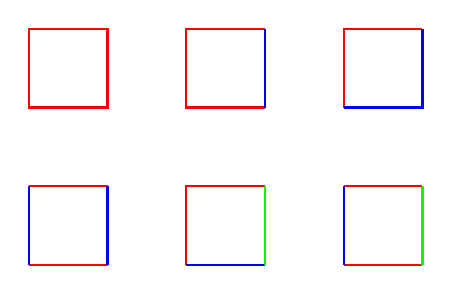
\begin{tikzpicture}

\coordinate (A) at (0,0);
\coordinate (B) at (0,-1);
\coordinate (C) at (1,-1);
\coordinate (D) at (1,0);

\coordinate (E) at (2,0);
\coordinate (F) at (2,-1);
\coordinate (G) at (3,-1);
\coordinate (H) at (3,0);

\coordinate (I) at (4,0);
\coordinate (J) at (4,-1);
\coordinate (K) at (5,-1);
\coordinate (L) at (5,0);

\coordinate (M) at (0,-2);
\coordinate (N) at (0,-3);
\coordinate (O) at (1,-3);
\coordinate (P) at (1,-2);

\coordinate (Q) at (2,-2);
\coordinate (R) at (2,-3);
\coordinate (S) at (3,-3);
\coordinate (T) at (3,-2);

\coordinate (U) at (4,-2);
\coordinate (V) at (4,-3);
\coordinate (W) at (5,-3);
\coordinate (X) at (5,-2);

\draw[color=red, thick] (A) -- (B) -- (C) -- (D) -- cycle;
\draw[color=red, thick] (H) -- (E) -- (F) -- (G);
\draw[color=blue, thick] (G) -- (H);
\draw[color=red,thick] (L) --(I) -- (J);
\draw[color=blue,thick] (J) --(K) -- (L);
\draw[color=red,thick] (M) -- (P);
\draw[color=red,thick] (N) -- (O);
\draw[color=blue,thick] (N) -- (M);
\draw[color=blue,thick] (O) -- (P);
\draw[thick,color=red] (T) -- (Q) -- (R);
\draw[thick,color=blue] (R) -- (S);
\draw[thick,color=green] (S) -- (T);
\draw[color=red,thick] (U) -- (X);
\draw[color=red, thick] (V) -- (W);
\draw[color=blue, thick] (V) -- (U);
\draw[color=green, thick] (W) -- (X);




  \end{tikzpicture}
\end{center}
\caption{De mulige kombinasjonene.}
\end{figure}

  \end{enumerate}
\end{losn}

\begin{oppg}
Beskriv banene for virkningen av $G$ på mengden av poler når $G$ er rotasjonsgruppen til tetraederet, oktaederet og ikosaederet.
\end{oppg}

\begin{losn}
Dette er ikke helt lett. Vi begynner med tetraederet.

\textbf{Tetraederet:} For hvert hjørne kan vi rotere ett hakk til venstre og ett hakk til høyre, og det er fire hjørner. Dermed får vi åtte symmetrier. Disse har poler i hjørnene til tetraederet og på diametralt motsatte sider. I tillegg kan vi rotere $180^\circ$ i en linje som går gjennom midtpunktene på motsatte kanter (tegn en tegning!). Dette gir tre nye mulige symmetrier. I tillegg har vi identitetssymmetrien. Til sammen har symmetrigruppa $12$ elementer. Legg merke til at polene kommer i tre grupper. Den ene gruppen er polene som svarer til hjørnene på tetraederet, og det er lett å se at gruppen virker transitivt på disse, så vi har én bane. I tillegg har vi de som er diametralt motsatt av hjørnene i tetraederet, og disse utgjør en bane. 

I tillegg har vi de seks hjørnene som svarer til linjene mellom kantene. Disse utgjør også én bane. Til sammen er det tre baner (dette kunne vi også regnet ut med formelen i forrige oppgave).

\textbf{Oktaederet:} Her hjelper det å ha en modell av oktaederet tilgjengelig (og kanskje en søkemotor som kan hjelpe deg å bekrefte at du har funnet alle rotasjonene...). For det første: i hvert gjørne kan vi rotere $90^\circ$. Rotasjonsaksen går gjennom et annet hjørne, så $3$ av de $6$ hjørnene bidrar med rotasjoner. Disse er på $90^\circ,180^\circ$ og $270^\circ$.  Vi har dermed $9$ rotasjoner i hjørner.

I tillegg kan vi sette en rotasjonsakse gjennom midtpunktene på motstående kanter og rotere $180^\circ$. Det er $12$ kanter, så vi får $6$ rotasjoner på $180^\circ$.

Til slutt kan vi rotere $120^\circ, 240^\circ$ i rotasjonsakser som går gjennom motstående flater. Det er åtte flater, så vi får $8/2 \cdot 2=8$ rotasjoner gjennom flater.

I tillegg har vi identitetstransformasjonen, så til sammen har vi $1+9+6+8=24$ elementer, og disse utgjør hele symmetrigruppen. Denne er også gjent som $S_4$, gruppen av symmetrier på $4$ ``symboler''.

Nå når vi vet gruppen er det ``lett'' å finne banene til polene. Polene er altså snittet av rotasjonsaksene med enhetssfæren, så de svarer til rotasjonene. Vi kan dermed snakke om ``orden'' til en pol: en pol har orden $n$ om $n$ er den største orden til en rotasjon med akse gjennom polen. Dermed ser vi at hjørnene til oktaederet ligger på poler av orden $4$, og at disse utgjør én bane. Det finnes også en bane bestående av poler av orden $2$, og en bane bestående av poler av tre (nemlig rotasjoner gjennom flatene). Dermed er det tre baner. 

\textbf{Ikosaederet: } Igjen: her hjelper det veldig å ha en modell foran seg (til nød en modell på datamaskin en kan rotere på). Vi har $6$ rotasjonsakser som går gjennom motstående hjørner (husk, det er $12$ hjørner i ikosaederet), hvor vi kan rotere $360^\circ/5 = 72^\circ$. Dette gir til sammen $4 \cdot 6=24$ rotasjoner. I tillegg kan vi rotere gjennom motstående kanter, og da $180^\circ$. Det er $15$ par av kanter, så vi får $15$ stykk $180^\circ$-rotasjoner. I tillegg kan vi rotere $120^\circ,240^\circ$ med rotasjonsakser gjennom par av motstående flater, og det blir derfor $2 \cdot 20/2=20$ slike rotasjoner.

Ved samme resonnering som over kommer vi til at det er tre baner. Den ene banen har $12$ elementer (hjørnene). Neste bane kommer fra $180^\circ$-rotasjonene, og disse svarer til kantene, så det er $30$ elementer i denne banen. Til slutt er det banen som svarer til flatene, og i denne er det $20$ elementer.
\end{losn}
\end{document}
